% !Mode:: "TeX:UTF-8"
\chapter[实验结果与性能分析]{实验结果与性能分析}[Experimental Results and Performance Analysis]\label{chap:Results}

\section[引言]{引言}

本章通过系统实验验证第三章和第四章提出的模板逆向攻击与模型反演攻击方法的有效性。实验内容包含三方面:在标准测试集上与现有代表性方法进行定量对比以评估攻击成功率与生成质量,考察方法在不同目标分类器架构上的泛化性能,以及通过消融实验量化各关键模块的性能贡献。

本章结构安排如下:第~\ref{sec:results_setup}~节介绍统一的实验配置与评估指标体系;第~\ref{sec:angular_diffusion_results}~节验证第三章提出的基于角度约束对比学习的模板逆向重建方法,报告白盒场景下的攻击性能并分析核心设计模块的作用;第~\ref{sec:progressive_training_results}~节验证第四章提出的基于换脸先验迁移的多目标自适应模型反演方法,对比不同分类器架构下的攻击效果并验证关键技术设计的合理性;第~\ref{sec:results_summary}~节对全章进行总结。

\section[实验配置与评估指标]{实验配置与评估指标}
\label{sec:results_setup}

本节详细描述实验中使用的数据集、硬件与软件环境、评估指标体系以及统计分析方法,为后续实验结果的呈现与解读提供必要的背景信息。

\subsection{数据集与训练配置}

本研究使用多个标准人脸数据集进行实验。VGGFace2~\cite{cao2018vggface2}数据集包含331万张图像覆盖9,131个身份,从中选取1000个类别作为目标分类器的私有训练数据,该部分数据严格隔离,不用于生成模型训练,以确保攻击评估的公平性。CelebA~\cite{liu2015deep}数据集包含202,599张人脸图像及40种属性标注,用作生成模型的辅助训练数据。FFHQ~\cite{karras2019style}数据集包含70,000张高质量人脸图像,与CelebA-HQ共同用于REFace基础模型的预训练。FaceScrub~\cite{ng2014data}数据集包含106,863张图像,作为MIA方法的辅助训练数据。LFW~\cite{huang2008labeled}数据集包含13,233张图像覆盖5,749个身份,MOBIO、AgeDB、IJB-C数据集分别包含不同场景和年龄段的人脸样本,这些数据集共同用于TIA方法攻击成功率的全面评估。

所有数据集均经过标准预处理流程处理。首先使用dlib~\cite{king2009dlib}工具检测人脸并提取5个关键点,计算相似变换矩阵将人脸对齐至标准姿态。然后中心裁剪完整面部区域,并根据模型需求缩放至相应分辨率:扩散模型使用$256\times256$分辨率,识别器使用$112\times112$分辨率。接着将像素值归一化至$[0,1]$或$[-1,1]$区间。在训练阶段,采用随机翻转、亮度对比度调整、高斯模糊等数据增强技术提升模型鲁棒性。对于TIA实验,使用ArcFace模型提取512维归一化模板向量,每个测试身份随机选取一张图像用于提取目标模板,其余图像用于评估生成质量。

针对第三章提出的基于角度约束对比学习的模板逆向重建方法,本研究基于EDM框架进行条件生成训练。训练采用批大小16,通过梯度累积技术达到有效批大小64。优化器选用AdamW,学习率设置为$1\times10^{-5}$并采用余弦退火调度策略,同时设置500步预热期以稳定训练初期。优化器的动量参数为$\beta_1=0.9$、$\beta_2=0.999$,权重衰减系数为$1\times10^{-4}$。为确保训练稳定性,采用两阶段训练策略:预热阶段仅优化像素空间去噪损失,建立基础生成能力;随后的主训练阶段引入完整的任务不确定性加权框架,初始化$\log\sigma_p = \log\sigma_f = 0$,使任务不确定性参数$\sigma_p$和$\sigma_f$作为可学习参数与网络参数同步更新,从而自动调整像素损失和特征损失的权重分配,实现像素质量与特征匹配的最优平衡。角度约束的裕度参数设置为$m=0.35$以对齐ArcFace的超球面特征空间,多样性约束权重$\beta=0.1$用于防止模式崩溃。ArcFace模板嵌入通过交叉注意力机制注入U-Net各层。推理阶段采用40步确定性采样生成图像。

针对第四章提出的基于换脸先验迁移的多目标自适应模型反演方法,本研究基于REFace换脸先验模型并结合LoRA微调技术实现。训练配置方面,批大小设置为8,通过梯度累积达到有效批大小32。采用AdamW优化器,其中LoRA模块的学习率设置为$5\times10^{-6}$,标签嵌入层学习率设置为$1\times10^{-4}$,两者均采用线性预热与余弦退火调度策略。优化器的动量参数为$\beta_1=0.5$、$\beta_2=0.999$,权重衰减系数为$1\times10^{-4}$。训练采用渐进式三阶段策略:阶段1仅使用真实图像条件预热标签嵌入层,建立身份嵌入向量到高质量换脸生成的映射能力;阶段2通过余弦退火调度实现从图像条件到标签条件的混合过渡,标签条件权重系数$\lambda(t)$从0逐渐增长至1.0;阶段3使用纯标签条件进行LoRA微调,适配换脸模型到目标分类器的嵌入空间。LoRA配置方面,秩设置为$r=16$,缩放系数为$\alpha=32$,应用于U-Net的注意力层和卷积层。LoRA矩阵$A$采用高斯分布初始化,$B$采用零初始化,并施加$L_2$正则化约束系数0.01以防止过拟合。损失函数方面,采用任务不确定性加权框架自动平衡五项优化目标:扩散先验损失保持生成质量,分类引导损失驱动攻击成功,特征中心正则化损失稳定优化轨迹,身份一致性损失确保语义连贯,感知质量损失提升视觉真实度。各项损失通过可学习的不确定性参数$\{\sigma_i\}$与网络参数联合优化,实现各任务相对权重的自动调整。标签嵌入层采用MLP结构,包含256维隐藏层,输出512维特征向量并进行$L_2$归一化。REFace基础模型在FFHQ与CelebA-HQ数据集上预训练获得。推理阶段采用DDIM采样器,设置噪声范围$\sigma_{\text{min}}=0.002$、$\sigma_{\text{max}}=80$,采样步数50步,并将LoRA增量权重合并至原始模型参数以简化推理流程。

\subsection{评估指标}

本研究建立了涵盖攻击成功率、生成质量与像素保真度的多维度评估指标体系,全面评估所提出方法的性能表现。


针对模板逆向攻击任务,采用以下指标评估重建图像的攻击有效性与生成质量:

(1)攻击成功率。衡量重建图像在被攻击的目标特征提取模型上成功通过身份验证的比例,即将重建图像输入提供原始模板的同一目标模型,计算其提取的特征与目标模板的相似度是否超过验证阈值。本研究在误识率为$10^{-2}$和$10^{-3}$两个阈值下报告攻击成功率,分别对应常规安全场景与高安全场景,攻击成功率越高表示攻击越成功。

(2)Fréchet Inception Distance,FID。衡量生成图像分布与真实图像分布的距离,该值越低表示分布越接近:
\begin{equation}
\text{FID} = \|\mu_r - \mu_g\|_2^2 + \text{Tr}(\Sigma_r + \Sigma_g - 2(\Sigma_r\Sigma_g)^{1/2})
\end{equation}

其中$\mu_r, \Sigma_r$和$\mu_g, \Sigma_g$分别为真实图像和生成图像在Inception-v3特征空间的均值与协方差。

(3)身份保持度。使用预训练ArcFace模型计算生成图像与目标身份真实图像之间的特征相似度,衡量身份信息的保留程度。计算方式为余弦相似度$\text{CosSim}(F(\hat{x}), F(x_{\text{target}}))$,该值越高表示身份保持越好。

针对模型反演攻击任务,采用以下指标评估攻击准确率与生成保真度:

(1)目标准确率与评估准确率。目标准确率衡量生成图像在目标分类器上的Top-1命中率,即分类器预测的Top-1类别与目标标签匹配的比例。由于人脸识别模型中存在相似度阈值,本研究要求生成的代表性样本超过此接受阈值以确保它们满足与私有图像相同的人脸距离要求。为了防止生成的图像仅仅满足目标模型而未能真正代表目标类别,本研究还计算交叉评估准确率,即使用一个独立的人脸识别模型来验证生成样本的准确率。目标准确率和评估准确率越高表示攻击越有效,两个指标共同反映攻击的有效性与代表性。

(2)FID。与模板逆向攻击任务相同,用于评估生成图像分布与真实训练数据分布的相似度。

(3)KNN距离。基于余弦相似度计算生成图像与目标类别真实图像在ArcFace特征空间中的K近邻平均相似度,反映生成图像与目标类别特征分布的接近程度。该距离越高表示生成图像与真实样本在特征空间中的相似性越强。

\subsection{实验设置与基准对比方法}

本研究在白盒攻击场景下开展实验,攻击者完全了解目标识别器和分类器的架构与参数,可以计算梯度进行优化,但无法访问模型的训练数据。

对于TIA实验,在MOBIO、LFW、AgeDB、IJB-C四个标准人脸数据集上评估攻击性能。每个测试身份随机选取一张图像通过ArcFace提取512维模板向量作为攻击输入,剩余图像用于计算SAR和ID-Pres指标。对比的基准方法包括NBNet系列~\cite{mai2018reconstruction}的四个变体NBNetA-M、NBNetA-P、NBNetB-M、NBNetB-P,Dong et al.~\cite{dong2021towards}基于优化的方法,Vendrow et al.~\cite{vendrow2021realistic}基于GAN的方法,Dong et al.~\cite{dong2023reconstruct}基于扩散模型的方法,GaFaR~\cite{shahreza2023template}采用特征对齐的方法,以及Shahreza et al.~\cite{10506232}的最新工作。

对于MIA实验,目标分类器在VGGFace2数据集的1000个类别上训练,从中随机选取100个类别进行攻击评估。攻击时仅使用类别标签,不使用该类别的任何图像。通过比较生成图像与目标类别真实图像的特征向量余弦相似度计算KNN距离。为验证跨架构泛化性,选择三种不同架构的目标分类器:ArcFace、IR152和Face.evoLVe。对比的基准方法包括GMI~\cite{zhang2020secret}基于生成对抗网络,FMI~\cite{khosravy2022model}利用特征匹配,PLG-MI~\cite{yuan2023pseudo}采用伪标签引导的条件生成对抗网络,以及Diff-MI~\cite{li2024diffmi}基于扩散模型的方法。

\section[模板逆向重建方法实验]{基于角度约束对比学习的模板逆向重建方法实验结果与分析}
\label{sec:angular_diffusion_results}

本节系统呈现和分析第三章提出的基于角度约束对比学习的模板逆向重建方法的实验结果。该方法采用EDM~\cite{karrasEluvidatingDiffusionModels2022}作为生成骨干,通过条件扩散过程从ArcFace特征模板重建高质量人脸图像。方法的核心包括:(1)角度约束特征损失,实现与ArcFace超球面几何的精确对齐;(2)任务不确定性加权框架,自动平衡去噪与特征匹配目标;(3)多样性约束机制,防止模式崩塌。本节从基准性能对比和消融实验等多个维度验证方法的有效性。

\subsection{基准性能评估}

本节的实验设置遵循第~\ref{sec:results_setup}~节所述的通用配置。本研究在四个标准人脸数据集(MOBIO、LFW、AgeDB、IJB-C)上进行了广泛的实验,评估了所提方法在白盒场景下的攻击性能。在白盒场景中,攻击者完全了解目标系统的特征提取器(ArcFace)架构与参数。

评估指标采用攻击成功率即重建图像在目标识别系统中成功通过身份验证的比例。实验分别在误识率为$10^{-2}$和$10^{-3}$的阈值下报告攻击成功率。

表~\ref{tab:tia_sota_comparison}展示了在不同FMR阈值下本文方法与现有方法的性能对比。对比方法包括NBNet~\cite{mai2018reconstruction}、Dong et al.~\cite{dong2021towards}、Vendrow et al.~\cite{vendrow2021realistic}、GaFaR~\cite{shahreza2023template}等。

\begin{table}[htbp]
  \centering
  \caption{不同TIA方法在不同FMR阈值下的攻击成功率(SAR, \%)对比}
  \label{tab:tia_sota_comparison}
  \resizebox{\textwidth}{!}{
  \begin{tabular}{lcccccccc}
    \hline
    \multirow{2}{*}{方法} & \multicolumn{4}{c}{FMR=$10^{-2}$} & \multicolumn{4}{c}{FMR=$10^{-3}$} \\
    \cmidrule(lr){2-5} \cmidrule(lr){6-9}
     & MOBIO & LFW & AgeDB & IJB-C & MOBIO & LFW & AgeDB & IJB-C \\
    \hline
    NBNetA-M~\cite{mai2018reconstruction} & 2.94 & 14.18 & 2.63 & 3.17 & 2.51 & 4.28 & 0.89 & 0.38 \\
    NBNetA-P~\cite{mai2018reconstruction} & 23.67 & 35.83 & 9.42 & 11.34 & 4.68 & 16.91 & 4.07 & 0.43 \\
    NBNetB-M~\cite{mai2018reconstruction} & 21.18 & 27.06 & 5.52 & 7.89 & 1.97 & 11.15 & 1.95 & 0.39 \\
    NBNetB-P~\cite{mai2018reconstruction} & 48.92 & 61.53 & 23.76 & 28.35 & 15.37 & 40.18 & 13.25 & 3.21 \\
    Dong et al.~\cite{dong2021towards} & 24.41 & 28.35 & 9.27 & 7.93 & 3.41 & 13.34 & 4.02 & 0.44 \\
    Vendrow et al.~\cite{vendrow2021realistic} & 69.38 & 77.15 & 44.62 & 38.51 & 29.18 & 57.84 & 29.78 & 7.56 \\
    Dong et al.~\cite{dong2023reconstruct} & 87.75 & 87.41 & 58.93 & 57.16 & 61.57 & 74.35 & 43.37 & 19.48 \\
    GaFaR~\cite{shahreza2023template} & 95.84 & 89.41 & 63.45 & 69.32 & 82.93 & 79.97 & 49.08 & 29.91 \\
    Shahreza et al.~\cite{10506232} & 96.53 & 92.47 & 73.91 & 78.62 & 84.89 & \textbf{85.14} & 60.18 & 45.57\\
    \hline
    Ours & \textbf{97.38} & \textbf{94.23} & \textbf{75.64} & \textbf{82.91} & \textbf{87.87} & 84.36 & \textbf{65.81} & \textbf{55.58} \\
    \hline
  \end{tabular}
  }
\end{table}

表~\ref{tab:tia_sota_comparison}展示本文方法与现有模板逆向攻击方法在四个基准数据集上的攻击成功率对比。在FMR=$10^{-2}$的常规安全场景下,本文方法在MOBIO、LFW、AgeDB和IJB-C上分别达到97.38\%、94.23\%、75.64\%和82.91\%,四项指标中的三项超越次优方法Shahreza et al.,平均攻击成功率达到87.54\%,较次优方法的85.38\%提升2.16个百分点。在FMR=$10^{-3}$的高安全场景下,本文方法在MOBIO、AgeDB和IJB-C上分别取得87.87\%、65.81\%和55.58\%,平均攻击成功率达到73.41\%,较次优方法的68.95\%提升4.46个百分点。

不同数据集上的性能差异体现了方法的适应性。在MOBIO受控环境数据集上,本文方法在两个FMR阈值下均获得最高攻击成功率,表明方法在标准化采集条件下的稳定性。在AgeDB年龄跨度数据集上,高安全场景下的65.81\%较次优方法提升5.63个百分点,验证了方法对面部特征变异的鲁棒性。在IJB-C无约束大规模数据集上,55.58\%的攻击成功率较次优方法提升10.01个百分点,充分证明方法在应对极端姿态、复杂光照和遮挡等非理想因素时的优势。在LFW数据集的FMR=$10^{-3}$测试中,本文方法获得84.36\%,略低于Shahreza et al.的85.14\%。该数据集主要包含网络爬取的高质量公众人物照片,其规范化姿态分布可能更适合基于高分辨率StyleGAN的方法。综合其他三个更具挑战性数据集的表现,本文方法展现出一致的性能优势。

方法的性能提升源于三方面协同作用。角度约束对比学习损失与ArcFace的余弦度量空间保持内在一致性,避免了欧氏距离度量在超球面特征空间中的几何失配,实现优化目标与识别器决策边界的精确对齐。任务不确定性加权框架通过可学习参数$\sigma_p$和$\sigma_f$动态平衡像素重建与特征匹配目标,根据训练进程自适应调整各任务权重,消除人工超参数调优的主观性。多样性正则化通过显式约束抑制特征空间的模式崩塌,确保生成分布在满足身份约束下保持样本多样性。

\subsection{消融实验}

为验证第三章提出的各关键模块的贡献,本节在LFW数据集上进行系统的消融实验。实验针对白盒攻击场景,目标模型为ArcFace。表~\ref{tab:tia_ablation}采用渐进式消融策略,从仅使用像素重建损失的基础模型开始,依次引入本文的三个核心设计:角度约束特征匹配(式~\ref{eq:tia_feat_loss})、任务不确定性加权框架(式~\ref{eq:tia_total_loss})和多样性正则化(式~\ref{eq:tia_diversity_loss}),量化每个模块的性能贡献。

\begin{table}[htbp]
  \centering
  \caption{模板逆向方法关键模块消融分析}
  \label{tab:tia_ablation}
  \begin{tabular}{lcccc}
    \hline
    模型配置 & SAR@$10^{-2}$ & SAR@$10^{-3}$ & FID & ID-Pres \\
    \hline
    $\mathcal{L}_{\text{pixel}}$ & 68.33\% & 41.67\% & 52.46 & 0.703 \\
    $\mathcal{L}_{\text{pixel}} + \mathcal{L}_{\text{feat}}$ & 91.33\% & 79.83\% & 32.18 & 0.891 \\
    + 任务不确定性加权 & 92.83\% & 82.17\% & 27.54 & 0.923 \\
    + $\mathcal{L}_{\text{div}}$  & 94.23\% & 84.23\% & 18.27 & 0.947 \\
    \hline
  \end{tabular}
\end{table}

消融实验结果定量揭示各核心模块对整体性能的渐进式贡献。基线配置仅采用像素重建损失时,高安全阈值下攻击成功率仅为41.67\%,表明单纯像素级监督不足以指导模型学习身份判别性特征。引入角度约束特征损失后,采用余弦相似度度量与ArcFace超球面几何精确对齐,攻击成功率显著提升至79.83\%,FID降至32.18,身份保持度达到0.891,验证了几何感知损失设计的有效性,证明优化目标与识别器决策边界对齐能在攻击性与生成质量两维度同时提升。

任务不确定性加权框架通过可学习参数$\sigma_p$和$\sigma_f$自动平衡像素重建与特征匹配权重,使攻击成功率进一步提升至82.17\%,FID优化至27.54,身份保持度提升至0.923,表明自适应权重调整能有效协调生成质量与攻击性之间的权衡关系。多样性正则化损失通过显式约束特征空间分布缓解模式崩塌,使攻击成功率达到84.23\%,FID降至18.27,身份保持度提升至0.947。从基线到完整模型配置,攻击成功率累计提升42.56个百分点,验证了各核心模块的有效性及协同作用。

\begin{figure}[htbp]
  \centering
  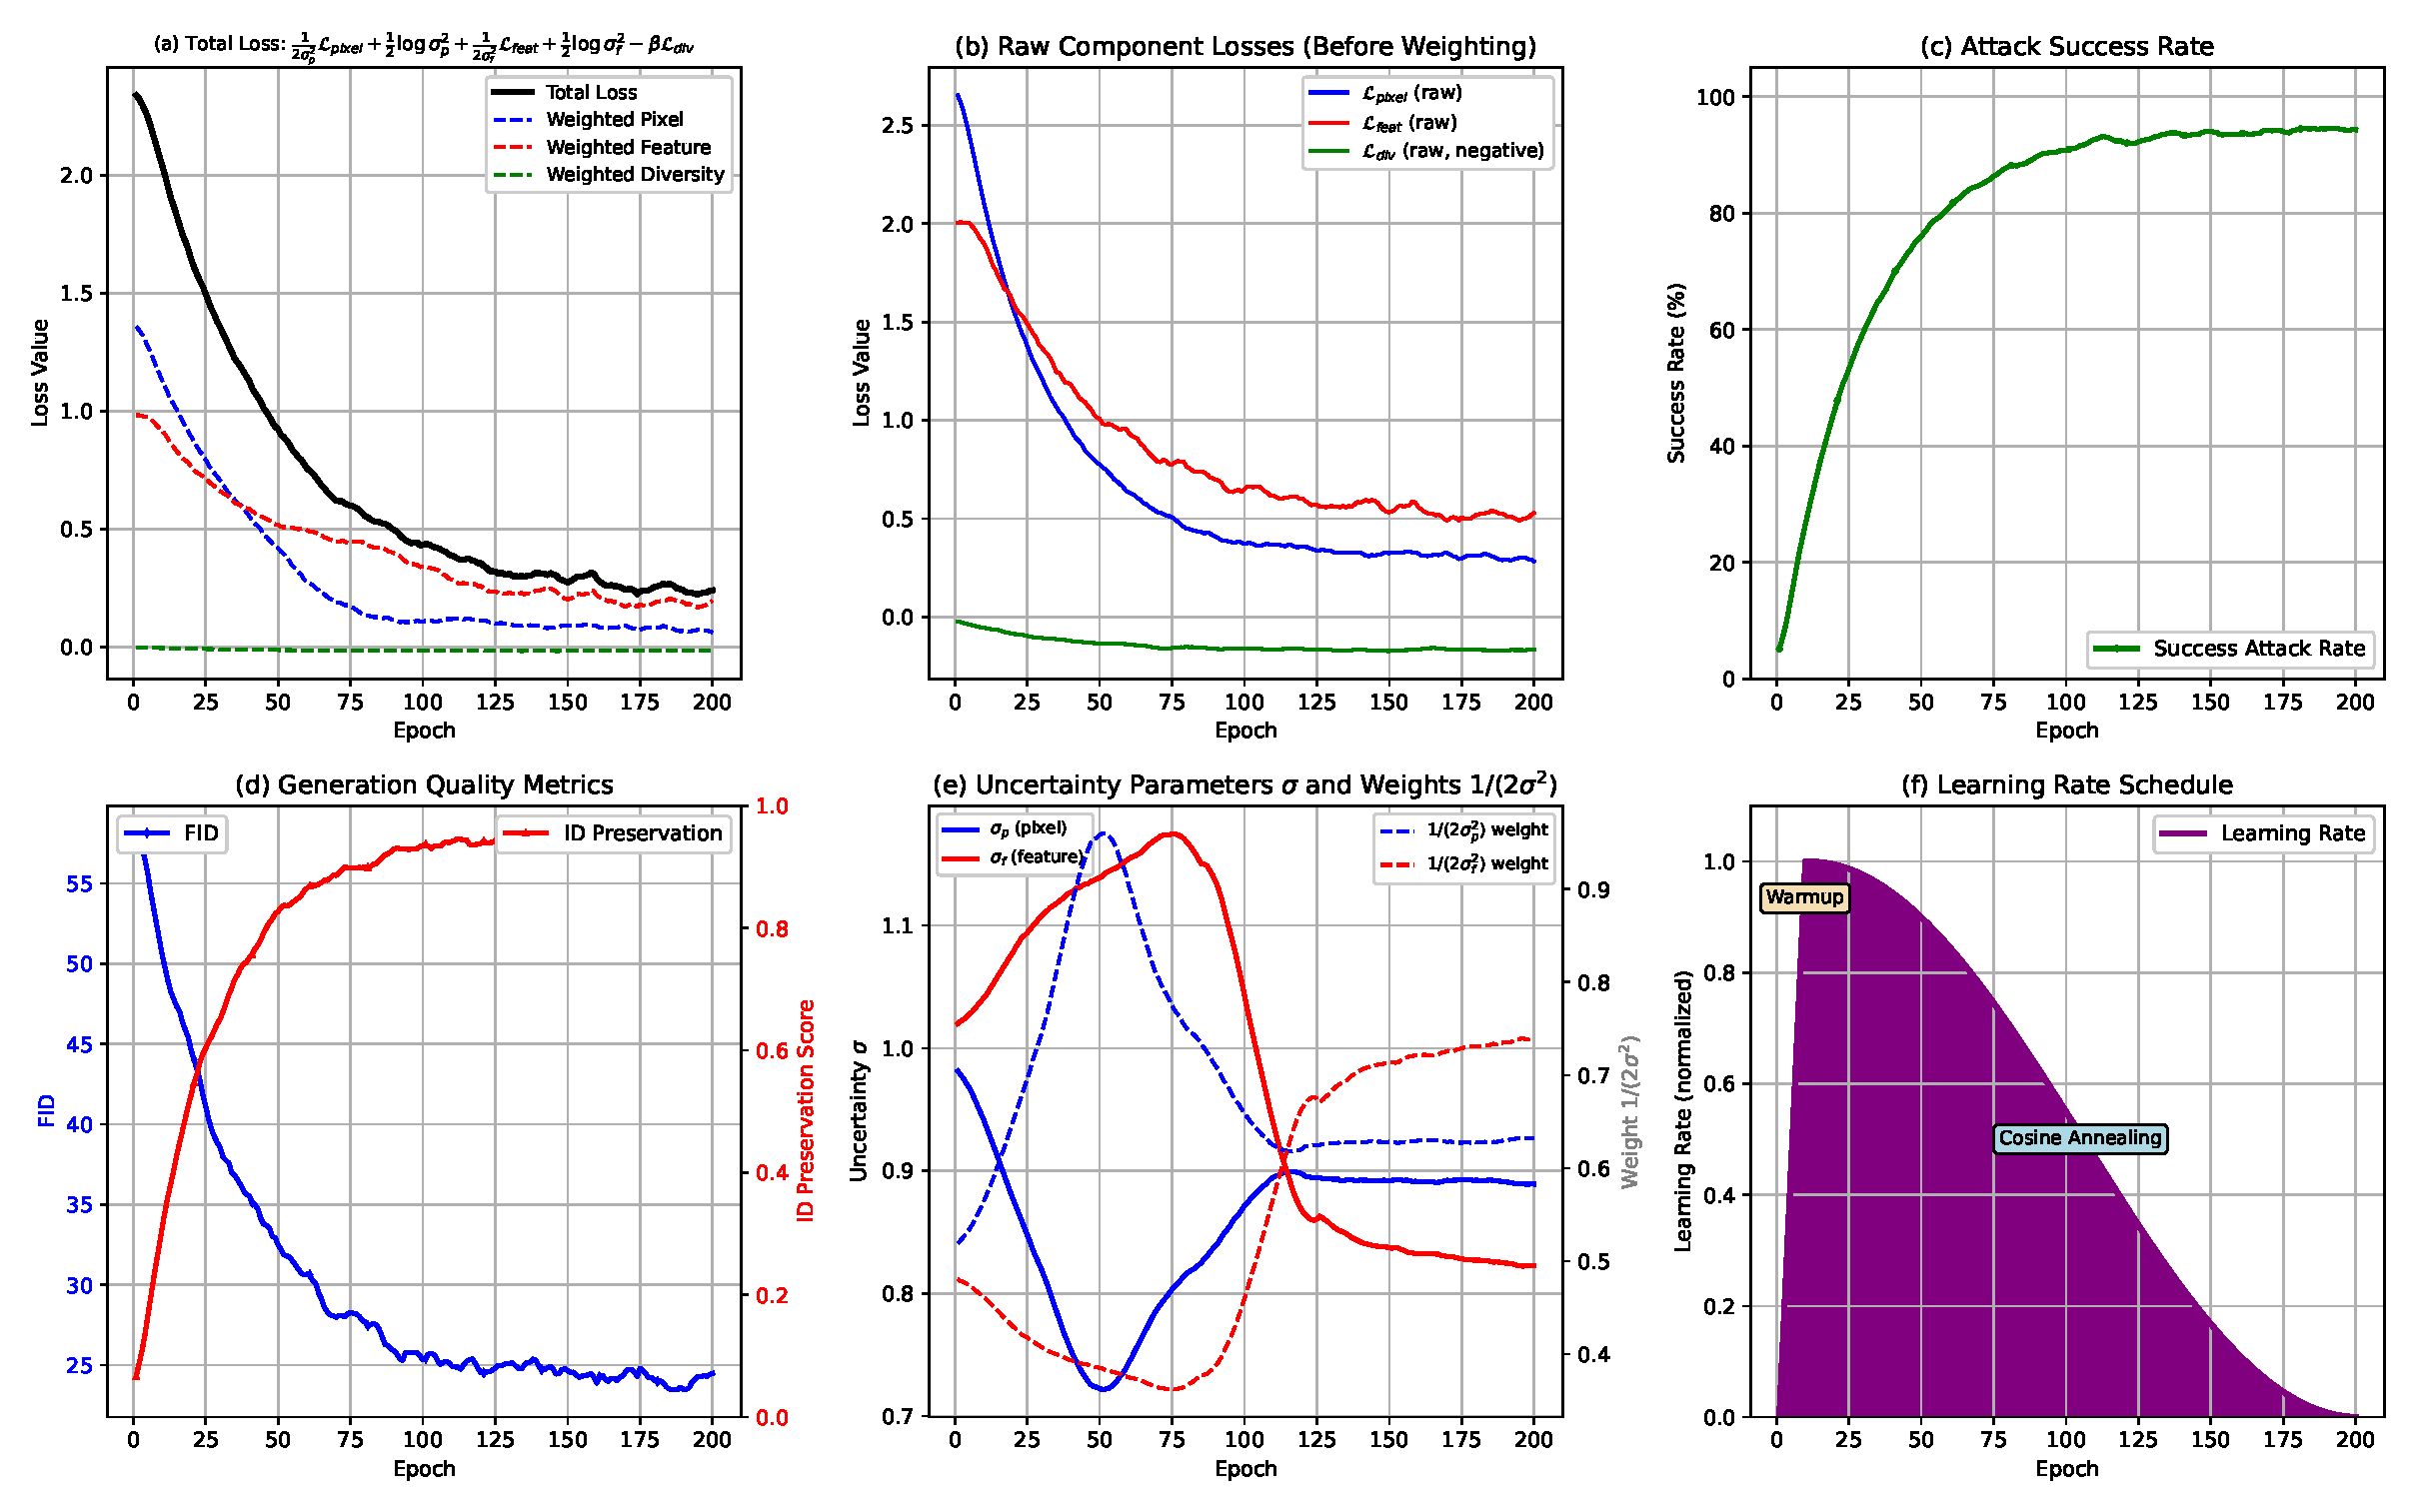
\includegraphics[width=0.95\textwidth]{figures/tia_training_curves.eps}
  \caption{TIA方法训练过程的损失与指标演化曲线}
  \label{fig:tia_training_curves}
\end{figure}

为深入理解模板逆向方法的学习过程,图~\ref{fig:tia_training_curves}展示了完整模型在CelebA数据集上训练200个epoch的主要损失曲线和评估指标演化。整体而言,各项指标呈现稳定收敛趋势,验证了方法的有效性。图中(a)展示总损失与加权损失的下降趋势,反映了多任务优化的协同效果;(b)呈现像素重建损失($\mathcal{L}_{\text{pixel}}$)和特征匹配损失($\mathcal{L}_{\text{feat}}$)的独立演化,两者在训练过程中持续下降并趋于稳定;(c)呈现攻击成功率(SAR)在不同FMR阈值下的提升过程,验证了方法的攻击有效性;(d)展示FID和身份保持度(ID-Pres)两项质量指标的变化,FID从初始值逐渐下降表明生成分布与真实分布的接近,ID-Pres的上升反映身份特征匹配度的提升;(e)展示不确定性参数$\sigma_p$、$\sigma_f$的演化,体现任务不确定性加权框架的自适应调整机制;(f)展示学习率的余弦退火调度过程。

任务不确定性加权机制的动态演化规律深刻揭示了该框架的自适应平衡能力。如图~\ref{fig:tia_training_curves}(e)所示,两个不确定性参数均从初始值$\sigma_p = \sigma_f = 1$开始演化。像素重建任务的不确定性参数$\sigma_p$下降至约0.7后逐渐回升至0.9并稳定,对应的权重系数$1/(2\sigma_p^2)$先增后减,该权重分配策略确保模型在训练初期优先建立基础的像素重建能力;特征匹配任务的不确定性参数$\sigma_f$则呈现先上升后下降的趋势,先增至约1.2再逐渐下降至0.82左右,其权重系数$1/(2\sigma_f^2)$在训练后期显著增大,该权重再分配过程反映了模型优化重心从底层生成能力向高层身份对齐能力的自适应转移机制。训练收敛后,$\sigma_f < \sigma_p$意味着特征匹配任务获得更高权重,符合模板逆向攻击的核心目标。该权重自动调整机制从根本上消除了人工超参数搜索的繁琐性,使模型能够在生成质量与攻击有效性之间实现动态最优平衡。从训练稳定性角度分析,各损失分量曲线在整个训练过程中未出现剧烈震荡或梯度爆炸等不稳定现象,该平滑的优化轨迹充分证明了EDM扩散框架与角度约束损失函数设计之间的良好兼容性。



\subsection{可视化结果与分析}

图~\ref{fig:tia_reconstruction}展示十个目标身份的模板重建结果。第一行为真实图像,第二行为从特征模板重建的图像,第三行为Grad-CAM生成的特征激活热力图。重建图像在面部结构、五官形态和整体身份特征与真实图像高度一致。热力图中红色高激活区域主要集中在眼睛、鼻子和嘴部等具有显著身份辨识度的区域,与人脸识别系统的特征提取模式相吻合,验证了角度约束特征匹配设计的有效性,说明方法成功实现了在超球面特征空间中的精准对齐。基于EDM框架生成的图像在细节纹理层面表现优异,皮肤质感、头发纹理、面部光影等精细特征均得到较好还原。

\begin{figure}[htbp]
  \centering
  \includegraphics[width=0.95\textwidth]{images/matrix_3x10.png}
  \caption{TIA方法的模板重建可视化}
  \label{fig:tia_reconstruction}
\end{figure}

上述可视化结果证明第三章提出的基于角度约束对比学习的模板逆向重建方法能够从抽象的特征模板重建出高质量且身份准确的面部图像,角度约束特征匹配、任务不确定性加权和多样性正则化等核心技术的协同作用使方法在攻击成功率与生成真实感之间实现有效平衡。

\section[模型反演攻击方法实验]{基于换脸先验迁移的多目标自适应模型反演方法实验结果与分析}
\label{sec:progressive_training_results}

本节系统呈现和分析第四章提出的基于换脸先验迁移的多目标自适应模型反演方法的实验结果。该方法的核心创新在于:(1)利用换脸模型的预训练先验进行迁移学习;(2)设计渐进式三阶段训练策略以实现平滑模态迁移;(3)构建任务不确定性加权的多目标优化框架以自动平衡多个优化目标。在技术实现上,方法通过标签条件嵌入层将类别标签映射为身份嵌入,并采用LoRA技术实现参数高效微调。本节通过基准性能评估、跨分类器泛化性分析、可视化结果展示以及关键模块消融实验等多个维度系统验证方法的有效性。

\subsection{基准性能评估}

本节的实验设置遵循第~\ref{sec:results_setup}~节所述的通用配置。目标分类器在VGGFace2数据集的1000个类别上训练,从中随机选取100个类别进行攻击评估。为验证方法的跨架构泛化能力,选择三种不同架构的目标分类器进行实验:ArcFace基于角度损失的度量学习,IR152采用改进残差网络,Face.evoLVe使用专门优化的识别架构。生成模型使用CelebA与FaceScrub数据集进行辅助训练,REFace基础模型在FFHQ与CelebA-HQ上预训练获得。为评估方法在分布偏移场景下的泛化性能,在AgeDB数据集上进行测试,该数据集的跨年龄分布特性提供了有效的分布外评估场景。

表~\ref{tab:mia_standard}对比了本文方法与四种现有代表性方法在三种目标分类器架构下的攻击性能。对比方法包括:GMI~\cite{zhang2020secret}基于生成对抗网络,FMI~\cite{khosravy2022model}利用特征匹配,PLG-MI~\cite{yuan2023pseudo}采用伪标签引导,Diff-MI~\cite{li2024diffmi}基于扩散模型。评估指标包括目标准确率(TarAcc)、评估准确率(EvalAcc)、生成保真度(FID)以及KNN距离(KNN Dist)。

\begin{table}[htbp]
  \centering
  \caption{不同目标分类器下的MIA攻击性能对比}
  \label{tab:mia_standard}
  \resizebox{\textwidth}{!}{
  \begin{tabular}{lcccccccccccc}
    \hline
    \multirow{2}{*}{Method} & \multicolumn{4}{c}{Target: ArcFace} & \multicolumn{4}{c}{Target: IR152} & \multicolumn{4}{c}{Target: Face.evoLVe} \\
    \cmidrule(lr){2-5} \cmidrule(lr){6-9} \cmidrule(lr){10-13}
     & TarAcc$\uparrow$ & EvalAcc$\uparrow$ & FID$\downarrow$ & KNN$\uparrow$ & TarAcc$\uparrow$ & EvalAcc$\uparrow$ & FID$\downarrow$ & KNN$\uparrow$ & TarAcc$\uparrow$ & EvalAcc$\uparrow$ & FID$\downarrow$ & KNN$\uparrow$ \\
    \hline
    GMI     & 28.52\% &  1.38\% & 24.87 & 0.5591    & 69.43\% & 10.85\% & 30.18 & 0.6652    & 71.92\% & 25.68\% & 41.07 & 0.7189 \\
    FMI     & 31.27\% & 21.63\% & 36.42 & 0.5308    & 54.16\% & 13.72\% & 41.25 & 0.7012    & 51.74\% & 18.85\% & 47.18 & 0.7436 \\
    PLG-MI  & 40.95\% & 16.87\% & 43.26 & 0.5793    & 83.52\% & 31.94\% & 48.65 & 0.7288    & 91.76\% & 29.43\% & 53.72 & 0.7658 \\
    Diff-MI & 94.18\% & 75.62\% & 29.53 & \textbf{0.7426}    & 93.75\% & 76.84\% & 32.68 & 0.8176    & \textbf{95.42}\% & 79.21\% & 36.47 & 0.8562 \\
    \hline
    Ours    & \textbf{94.87\%} & \textbf{83.15\%} & \textbf{23.26} & 0.7165  & \textbf{93.28\%} & \textbf{84.23\%} & \textbf{25.83} & \textbf{0.8534}    & 94.38\% & \textbf{82.94\%} & \textbf{26.91} & \textbf{0.9024} \\
    \hline
  \end{tabular}
  }
\end{table}

表~\ref{tab:mia_standard}展示本文方法在三种目标分类器架构下的攻击性能。在ArcFace目标分类器上,本文方法达到94.87\%目标准确率和83.15\%评估准确率,FID为23.26,KNN距离为0.7165。对比Diff-MI的94.18\%目标准确率和75.62\%评估准确率,本文方法在评估准确率上提升7.53个百分点,FID降低6.27,表明生成样本不仅能攻击目标模型,更能真正代表目标类别特征,在独立评估模型上保持高识别率。在IR152和Face.evoLVe分类器上,本文方法同样在评估准确率和FID上展现一致优势,评估准确率分别达到84.23\%和82.94\%,FID分别为25.83和26.91,均优于所有基准方法。

跨架构性能分析验证了方法的泛化能力。三种分类器采用不同网络架构和训练策略,ArcFace基于角度损失的度量学习,IR152基于改进残差网络,Face.evoLVe使用专门优化的识别架构。在所有架构上,本文方法在评估准确率、FID和KNN距离指标上保持显著优势,表明基于REFace的生成先验能有效适应不同特征空间,通过LoRA微调精准拟合不同架构的特征分布。评估准确率在所有架构上均超过82\%,显著高于Diff-MI的75-79\%,证明生成样本具有强泛化能力。虽然在Face.evoLVe分类器上的目标准确率(94.38\%)略低于Diff-MI(95.42\%),但本文方法在评估准确率上的显著优势(82.94\% vs. 79.21\%)表明生成样本更能真实代表目标类别特征。方法仅需微调LoRA参数即可在所有架构上取得稳定高质量重建,验证了标签条件嵌入层设计的有效性和参数高效性。

\subsection{消融实验}

为量化第四章提出的各关键设计模块的贡献,本节在VGGFace2数据集上训练的ArcFace目标分类器上进行系统的消融实验。实验从两个维度评估:渐进式三阶段训练策略的作用,以及各损失项的性能贡献。
\begin{table}[htbp]
  \centering
  \caption{模型反演方法渐进式训练策略消融实验}
  \label{tab:mia_training_ablation}
  \begin{tabular}{lccccc}
    \hline
    训练策略 & TarAcc & EvalAcc & FID & KNN Dist \\
    \hline
    单阶段 (直接标签条件) & 70.85\% & 63.74\% & 43.21 & 0.4687 \\
    两阶段 (图像预热$\rightarrow$标签) & 88.92\% & 78.56\% & 32.45 & 0.6254 \\
    三阶段 (图像$\rightarrow$混合$\rightarrow$标签) & 94.87\% & 83.15\% & 23.26 & 0.7165 \\
    \hline
  \end{tabular}
\end{table}

表~\ref{tab:mia_training_ablation}对比不同训练策略对攻击性能的影响。直接使用随机初始化标签嵌入的单阶段训练,目标准确率仅为70.85\%,评估准确率63.74\%。引入图像预热的两阶段训练,通过真实图像建立身份嵌入到换脸生成的映射,目标准确率提升至88.92\%,评估准确率78.56\%。采用混合条件过渡的三阶段训练,通过余弦退火实现从图像到标签的平滑模态转换,目标准确率达到94.87\%,评估准确率83.15\%,较单阶段分别提升24.02和19.41个百分点,FID降至23.26,KNN距离达到0.7165,验证了平滑模态迁移对实现高质量模型反演的关键作用。


\begin{figure}[htbp]
  \centering
  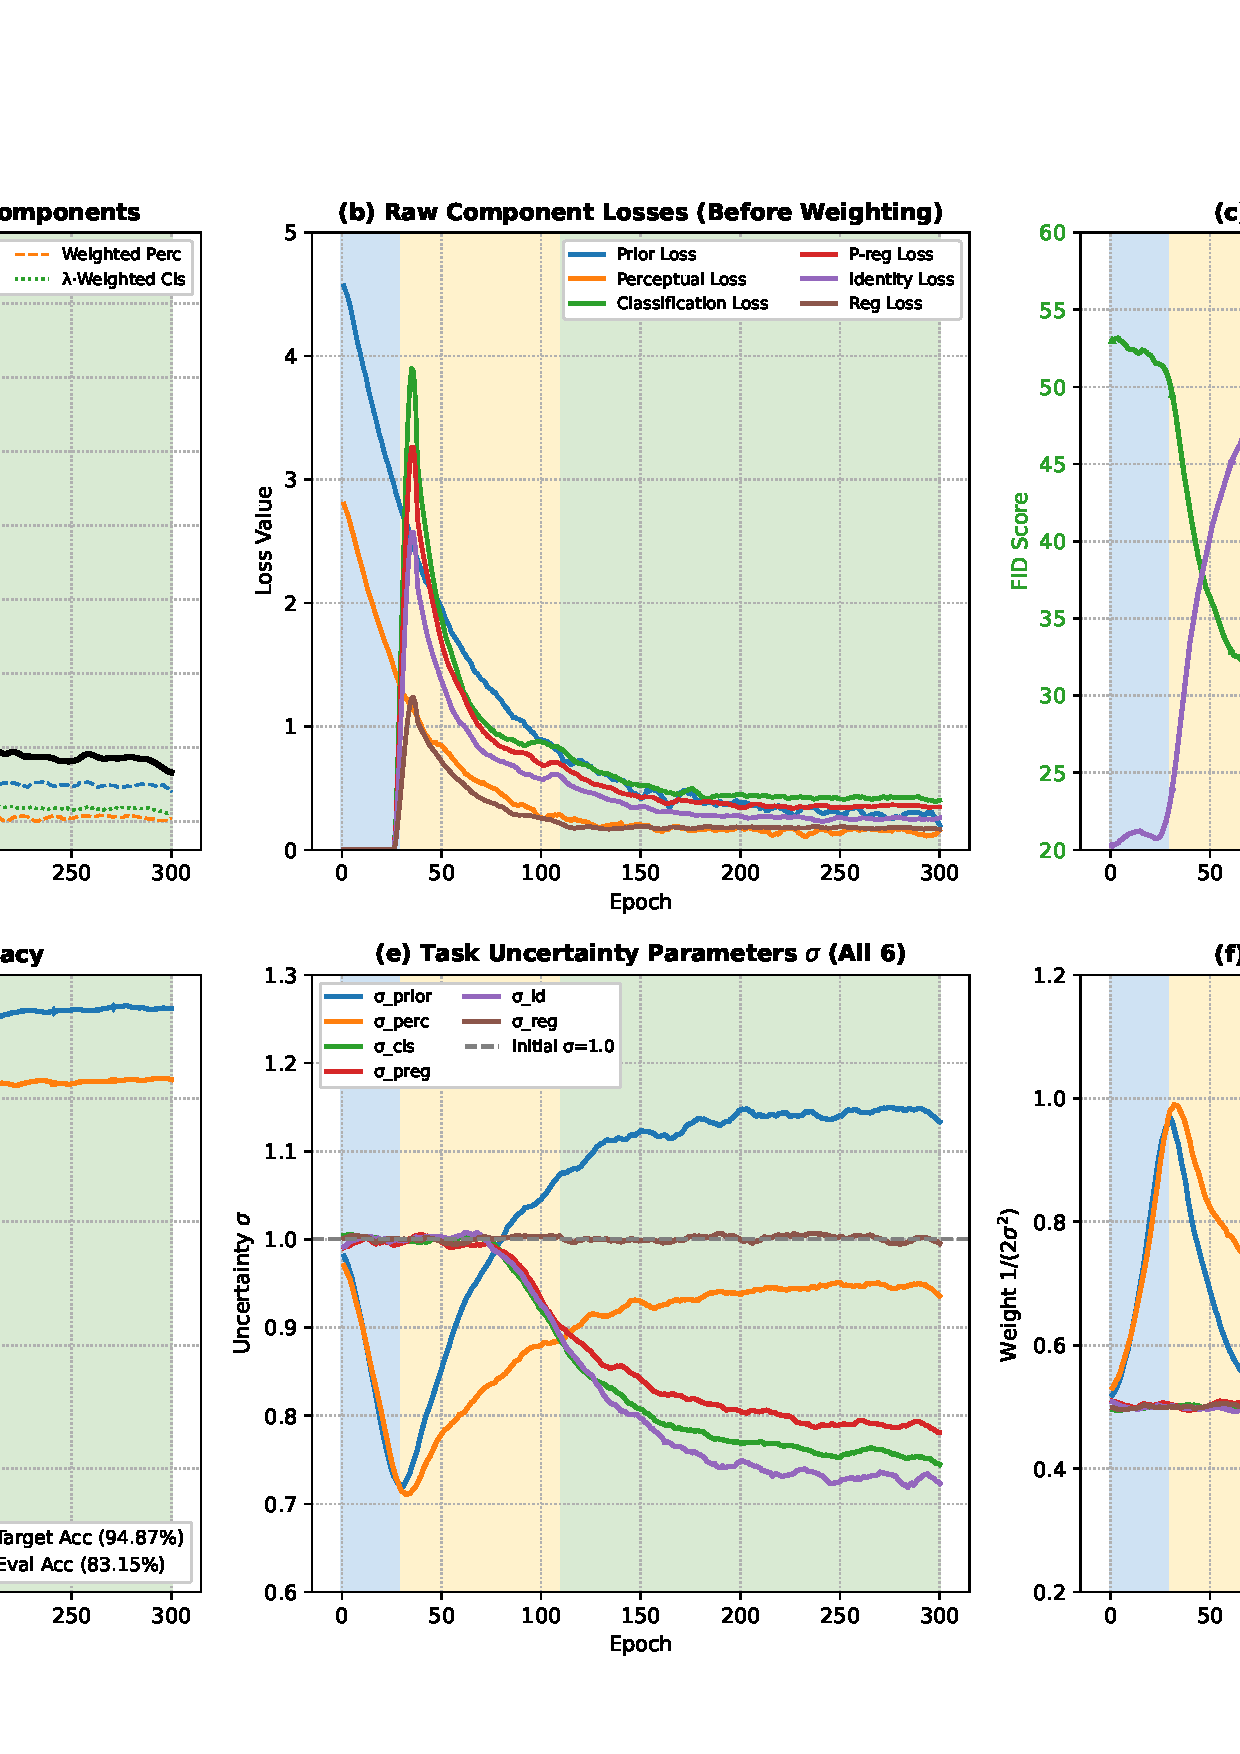
\includegraphics[width=\textwidth]{figures/mia_training_curves.pdf}
  \caption{MIA方法三阶段渐进式训练过程的损失与指标演化曲线}
  \label{fig:mia_training_curves}
\end{figure}
图~\ref{fig:mia_training_curves}展示三阶段训练的损失与指标演化。图中背景色区分训练阶段:阶段1(蓝色)为图像条件预热,阶段2(黄色)为混合条件过渡,阶段3(绿色)为纯标签条件适配。子图(a)展示总损失与部分核心损失的演化趋势,反映整体优化效果;子图(b)呈现全部损失项的独立演化,验证各损失函数的收敛性。子图(c)显示FID和KNN距离两项质量指标的变化,在阶段1图像条件预热阶段,由于仅建立图像到换脸的基础映射而未针对目标类别优化,FID维持在较高水平,KNN距离保持在极低值几乎无变化;阶段2引入标签条件后,随着混合系数$\lambda(t)$从0逐渐增长至1,标签条件的贡献逐步增强,两项指标开始显著改善,FID快速下降,KNN距离大幅跃升,充分体现了标签条件引导对目标类别特征匹配的关键作用;阶段3通过LoRA微调进一步优化,两项指标持续提升直至收敛,最终达到表~\ref{tab:mia_training_ablation}所示的三阶段训练结果。子图(d)展示目标准确率和评估准确率的提升过程,呈现与质量指标相似的演化规律。在阶段1,由于尚未建立标签到嵌入的映射,两项准确率保持在极低水平;阶段2引入标签条件后,准确率快速上升;阶段3进一步提升,最终收敛至表~\ref{tab:mia_training_ablation}的三阶段训练策略对应值。子图(e)展示任务不确定性参数$\sigma_i$的动态演化,扩散先验的$\sigma_{\text{prior}}$在阶段1保持较低水平确保生成质量,分类引导和身份一致性的$\sigma_{\text{cls}}$、$\sigma_{\text{id}}$在阶段2-3显著下降驱动攻击准确率提升;子图(f)展示对应的权重系数$1/(2\sigma_i^2)$的变化,清晰反映各任务重要性的自适应调整过程,该自动权重调整机制使框架无需人工超参数搜索即可在多目标间达到动态均衡。


\begin{table}[htbp]
  \centering
  \caption{模型反演方法损失项组合消融实验}
  \label{tab:mia_loss_ablation}
  \begin{tabular}{lcccc}
    \hline
    损失组合 & TarAcc & EvalAcc & FID & KNN Dist \\
    \hline
    仅扩散先验 $\mathcal{L}_{\text{prior}}$ & 7.85\% & 5.92\% & 53.47 & 0.4156 \\
    + 分类引导 $\mathcal{L}_{\text{cls}}$ & 77.24\% & 70.38\% & 36.82 & 0.5387 \\
    + 身份一致性 $\mathcal{L}_{\text{id}}$ & 92.56\% & 79.47\% & 29.15 & 0.6743 \\
    + 感知质量 $\mathcal{L}_{\text{perc}}$ & 94.87\% & 83.15\% & 23.26 & 0.7165 \\
    \hline
  \end{tabular}
\end{table}

表~\ref{tab:mia_loss_ablation}展示不同损失项组合对性能的影响。仅使用扩散先验损失时,缺乏针对目标分类器的优化信号,目标准确率仅为7.85\%。引入分类引导损失后,目标准确率显著提升至77.24\%。添加身份一致性损失,目标准确率达到92.56\%,评估准确率79.47\%。引入感知质量损失后,目标准确率达到94.87\%,评估准确率83.15\%,FID降至23.26。每增加一个损失项,评估准确率提升幅度均大于目标准确率,特别是身份一致性损失带来显著提升,表明这些损失项不仅提高攻击成功率,更增强生成样本的真实代表性和泛化能力,验证了多目标优化框架的必要性。


\subsection{可视化结果与分析}

为直观展示模型反演方法的生成质量与多样性,图~\ref{fig:mia_grid_by_target}展示了针对不同目标类别的模型反演结果。其中每行对应一个源人脸,每列对应一个目标类别。该图验证了方法在固定源人脸条件下跨多个目标类别的攻击能力和生成多样性。从图中可观察到:同一行的生成图像继承了源人脸的姿态和表情属性,但在关键身份特征如面部轮廓、五官比例、发型等方面已转换为目标身份特征;同一列的生成图像虽源于不同源人脸,但在目标身份的视觉特征上保持高度一致,证明标签条件嵌入层成功学习目标类别身份表征。不同源人脸展现丰富的姿态变化、表情变化和光照条件,验证方法在不同源人脸条件下的鲁棒性。源人脸的姿态和表情属性被准确保留并迁移至目标身份,验证基于REFace的换脸先验能为模型反演任务提供强大结构引导,显著提升生成质量。

\begin{figure}[htbp]
  \centering
  \includegraphics[width=0.95\textwidth]{images/grid_by_target.jpg}
  \caption{模型反演方法针对不同目标类别的生成样本可视化。}
  \label{fig:mia_grid_by_target}
\end{figure}

生成图像不仅被目标分类器正确识别为对应类别,同时在视觉质量上呈现良好真实感,包括自然的肤色分布、清晰的五官轮廓以及合理的面部结构比例。利用REFace换脸先验显著提升生成质量,预训练的换脸模型为生成过程提供强大面部几何先验知识,使生成图像在面部结构一致性和光照自然度方面表现优异。标签条件嵌入层通过MLP网络成功实现从离散类别标签到连续身份表示空间的映射,不同类别的生成图像呈现明显身份区分度,验证标签条件嵌入机制的有效性。

上述可视化结果验证第四章提出的基于换脸先验迁移的多目标自适应模型反演方法在保持高攻击准确率的同时能显著提升重建图像的保真度和视觉质量,基于换脸先验的生成框架与标签条件嵌入机制的有机结合使方法在攻击有效性与生成真实感之间实现良好平衡,展现出在实际应用场景中的潜在威胁性。

\section[本章小结]{本章小结}
\label{sec:results_summary}

本章通过系统实验验证了本文提出的模板逆向攻击与模型反演攻击方法的有效性,并深入分析了关键技术组件的作用。

针对模板逆向攻击任务,实验结果表明第三章提出的基于角度约束对比学习的方法在白盒场景下实现了高成功率的模板重建。在误识率为$10^{-3}$的高安全场景下,该方法在MOBIO、AgeDB和IJB-C数据集上分别达到87.87\%、65.81\%和55.58\%的攻击成功率,平均攻击成功率73.41\%较次优方法提升4.46个百分点。在LFW数据集上,FID为18.27。消融实验验证了角度约束特征匹配在超球面特征空间中的优势,任务不确定性加权机制能够自动平衡像素质量与特征匹配,多样性正则化有效避免了模式崩塌,这些核心设计的协同作用使方法能够从有限的模板向量生成高保真度人脸图像。

针对模型反演攻击任务,实验证实第四章提出的基于换脸先验迁移的方法在攻击准确率和生成保真度之间取得了良好平衡。在ArcFace目标分类器上,该方法达到94.87\%目标准确率和83.15\%评估准确率,FID为23.26。该方法在IR152和Face.evoLVe分类器上均表现稳定,验证了其跨架构泛化能力。消融实验揭示了渐进式三阶段训练策略的重要性,该策略通过逐步过渡实现了从图像条件到标签条件的平稳转换。LoRA参数高效微调技术使方法仅需微调极少比例参数即可达到接近全参数微调的效果,显著降低了计算和存储开销。任务不确定性加权框架自动平衡了扩散先验、分类引导、身份一致性、感知质量和正则化五个优化目标,避免了繁琐的超参数调试过程。

本章实验全面验证了所提方法的有效性和泛化性。实验结果不仅揭示了人脸识别系统面临的隐私泄露风险,也为防御机制的设计提供了实证依据,对于推动隐私保护技术的发展具有重要的理论和实践意义。

% Local Variables:
% TeX-master: "../main"
% TeX-engine: xetex
% End:
